% ===== BLOCO 1 — METODOLOGIA (com todos os gráficos) =====
\section{Metodologia}
\label{sec:metodologia}

\subsection{Fonte de dados}
O conjunto de dados utilizado é o \textit{Air Quality UCI}~\cite{Vito2008}, disponibilizado pelo UCI Machine Learning Repository. O conjunto compreende aproximadamente 9\,358 observações horárias capturadas entre março de 2004 e fevereiro de 2005 por um dispositivo multisensor instalado ao nível do solo em uma área urbana italiana. As variáveis incluem leituras de cinco sensores MOx (PT08.S1--PT08.S5), medições de referência para poluentes (por exemplo, CO, NOx, NO2, C6H6) e variáveis meteorológicas (temperatura -- T, umidade relativa -- RH, umidade absoluta -- AH). Valores ausentes originais no dataset foram marcados com \texttt{-200} e tratados conforme descrito na Seção~\ref{sec:preproc}.

\subsection{Pré-processamento}
\label{sec:preproc}
As etapas de pré-processamento foram:
\begin{enumerate}
    \item \textbf{Leitura e conversão de datas:} as colunas \texttt{Date} e \texttt{Time} foram combinadas em um único índice \texttt{datetime} e convertidas para tipo \texttt{datetime}.
    \item \textbf{Substituição de marca de ausentes:} os valores iguais a \texttt{-200} foram substituídos por \texttt{NaN}.
    \item \textbf{Remoção de colunas e observações:} conforme regra explícita do trabalho, variáveis com perda de informação superior a \(90\%\) foram descartadas (por exemplo, \texttt{NMHC(GT)}) e observações duplicadas foram removidas.
    \item \textbf{Tratamento de ausentes:} para análises descritivas e PCA adotou-se \emph{listwise deletion} apenas nas etapas em que a matriz não podia conter \texttt{NaN} (por exemplo, cálculo de covariância para PCA). Para visualizações e algumas estatísticas foram mantidas observações com \texttt{NaN} para evidenciar a extensão do problema.
    \item \textbf{Padronização:} variáveis numéricas de preditores foram padronizadas (z-score) antes da aplicação da PCA e de alguns testes paramétricos.
\end{enumerate}

\subsection{Sumário do dataset e valores ausentes}
Para facilitar a leitura, a Tabela~\ref{tab:missing} lista as variáveis selecionadas e a percentagem de valores ausentes observada no processamento:

\begin{table}[htbp]
    \centering
    \caption{Contagem de valores ausentes (em \%) — principais variáveis.}
    \label{tab:missing}
    \begin{tabular}{lrr}
        \hline
        \textbf{Variável} & \textbf{Ausentes (n)} & \textbf{Ausentes (\%)} \\
        \hline
        NMHC(GT)         & 8\,557 & \(90.35\%\) \\
        CO(GT)           & 1\,797 & \(18.97\%\) \\
        NO2(GT)          & 1\,756 & \(18.54\%\) \\
        NOx(GT)          & 1\,753 & \(18.51\%\) \\
        PT08.S1(CO)      & 480    & \(5.07\%\) \\
        PT08.S2(NMHC)    & 480    & \(5.07\%\) \\
        C6H6(GT)         & 480    & \(5.07\%\) \\
        PT08.S3(NOx)     & 480    & \(5.07\%\) \\
        PT08.S4(NO2)     & 480    & \(5.07\%\) \\
        PT08.S5(O3)      & 480    & \(5.07\%\) \\
        T (Temperatura)  & 480    & \(5.07\%\) \\
        RH (Umid. rel.)  & 480    & \(5.07\%\) \\
        AH (Umid. abs.)  & 480    & \(5.07\%\) \\
        \hline
    \end{tabular}
\end{table}

\noindent\textbf{Interpretação:} a alta fração de ausentes em \texttt{NMHC(GT)} motivou sua exclusão de análises agregadas e do índice composto de poluição; as demais variáveis apresentaram perda moderada e foram mantidas, com atenção à técnica de análise (procedimentos que exigem matriz completa usaram exclusão de linhas).

\subsection{Engenharia de atributos e definição de classes}
\label{sec:features}
\begin{itemize}
    \item \textbf{Índice de Poluição Composto (CPI):} poluentes de referência (\texttt{CO(GT)}, \texttt{NOx(GT)}, \texttt{NO2(GT)}, \texttt{C6H6(GT)}) foram padronizados (z-score) e agregados pela média das z-scores.
    \item \textbf{Classes de poluição:} o CPI foi discretizado em três quantis (\textit{Low}, \textit{Moderate}, \textit{High}) para análises condicionais.
    \item \textbf{Atributos temporais:} extraíram-se \texttt{month}, \texttt{weekday} e \texttt{day\_period} (\texttt{ngt, mng, aft, eve}) para investigar sazonalidade diária e semanal.
\end{itemize}

\subsection{Análise exploratória (EDA) e visualizações}
\begin{figure}[htbp]
    \centering
    
\includegraphics[width=0.95\linewidth]{figures/histograms_univariate_selected.png}
    \caption{Histogramas univariados — seleção de variáveis. Distribuições assimétricas com caudas longas em poluentes sugerem picos esporádicos; a densidade suavizada realça a não normalidade.}
    \label{fig:histograms}
\end{figure}

\paragraph{Boxplots e outliers.}
A Figura~\ref{fig:boxplots_selected} apresenta boxplots das variáveis selecionadas (\texttt{NOx(GT), C6H6(GT), PT08.S3(NOx), PT08.S2(NMHC), T, RH}). \textbf{Interpretação:} evidenciam-se \emph{outliers} extremos, assimetria e amplitudes distintas entre sensores e variáveis meteorológicas; tal padrão sugere estatísticas robustas e, em modelagem, eventual winsorização.

\begin{figure}[htbp]
    \centering
    
\includegraphics[width=0.85\linewidth]{figures/boxplot_selected.png}
    \caption{Boxplots — subconjunto de preditores e variáveis meteorológicas.}
    \label{fig:boxplots_selected}
\end{figure}

\paragraph{Série temporal resumida e distribuições.}
A Figura~\ref{fig:summary_selected} combina séries temporais, histogramas e boxplots compactos para colunas selecionadas, permitindo avaliar lacunas temporais e padrões sazonais.

\begin{figure}[htbp]
    \centering
    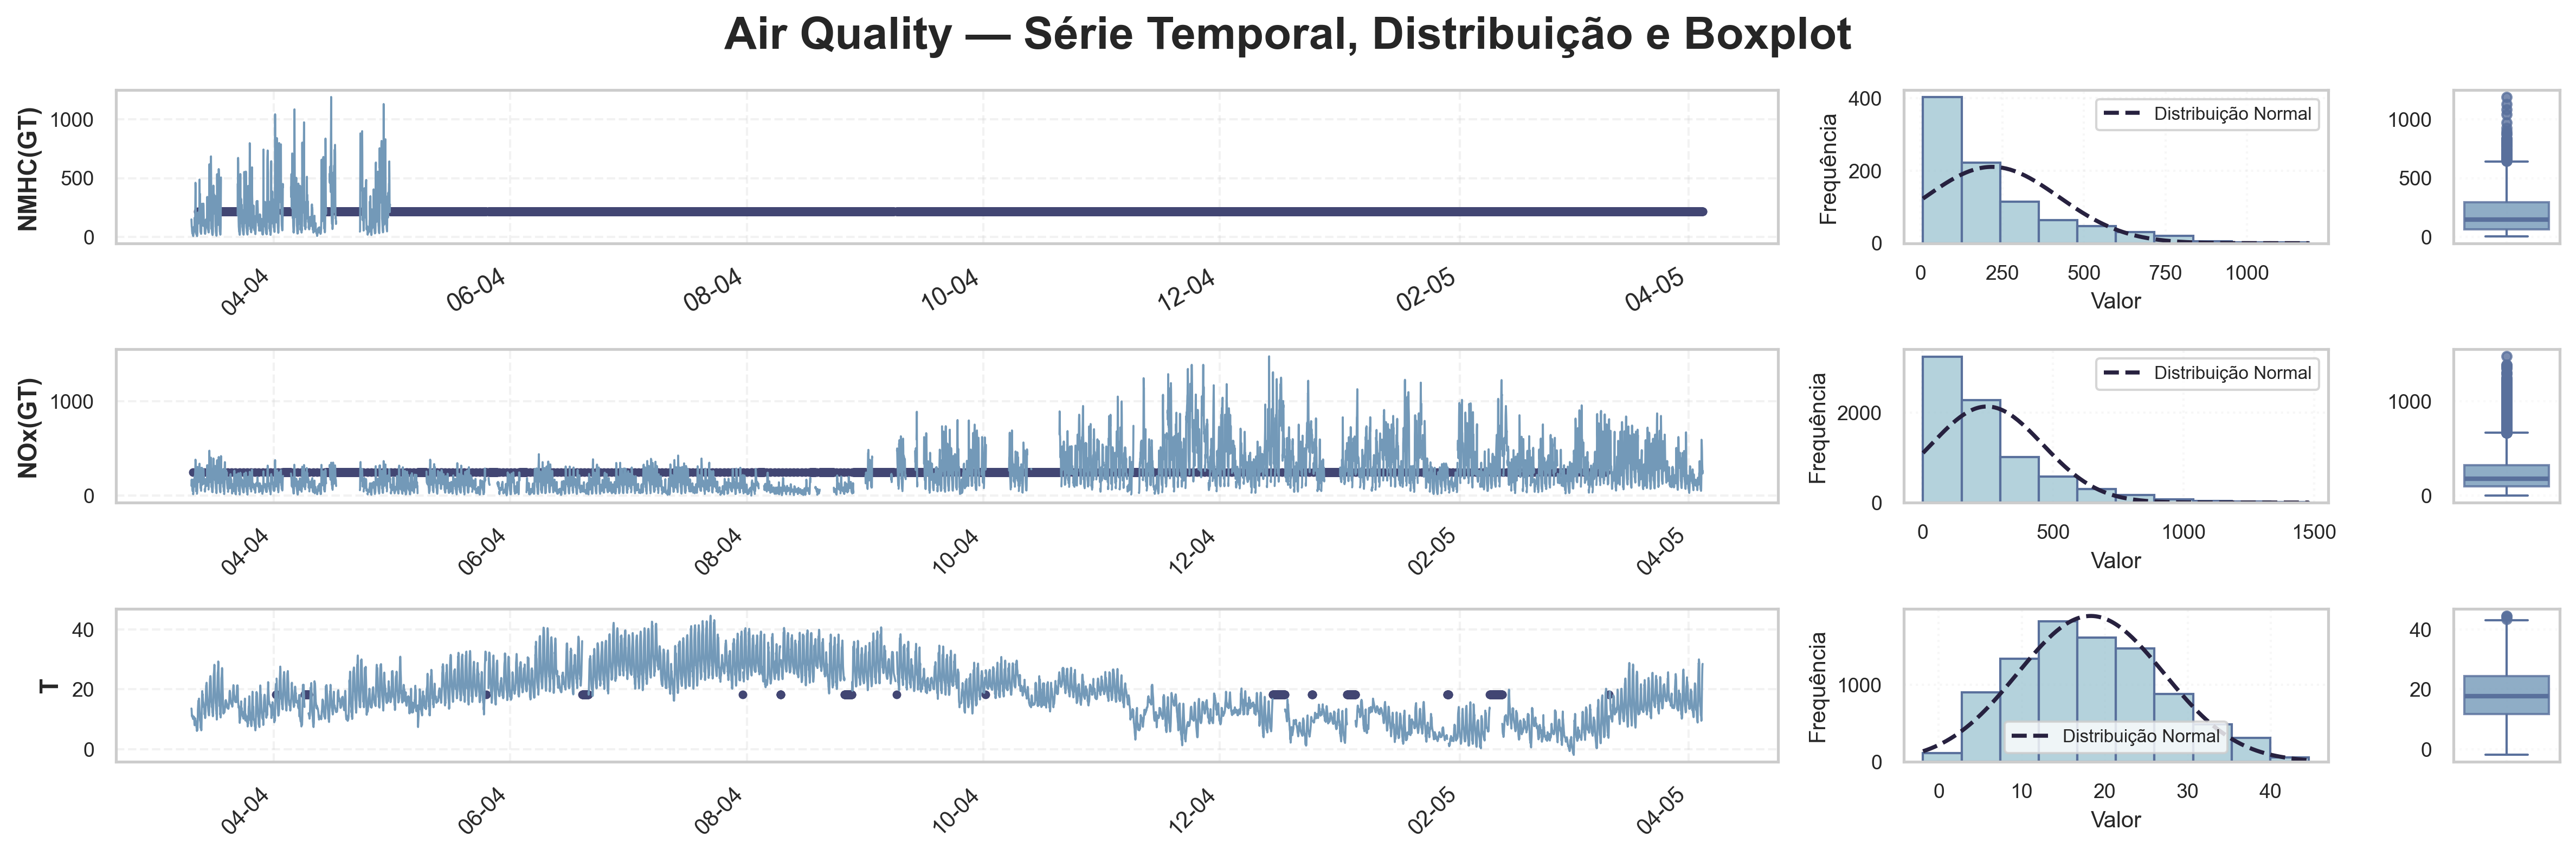
\includegraphics[width=0.95\linewidth]{figures/air_quality_summary_selected.png}
    \caption{Séries temporais, histogramas e boxplots (seleção). Notar pontos que marcam valores ausentes e variações mensais.}
    \label{fig:summary_selected}
\end{figure}

\paragraph{Distribuições condicionadas por classes e por tempo.}
As visualizações estratificadas por classe de poluição e por recortes temporais mostram deslocamentos de nível em sensores correlacionados a NOx/NO2 e padrões sazonais coerentes com meteorologia.

\paragraph{Matriz de correlação.}
A Figura~\ref{fig:corr} apresenta a matriz de correlação de Pearson entre preditores numéricos.

\begin{figure}[htbp]
    \centering
    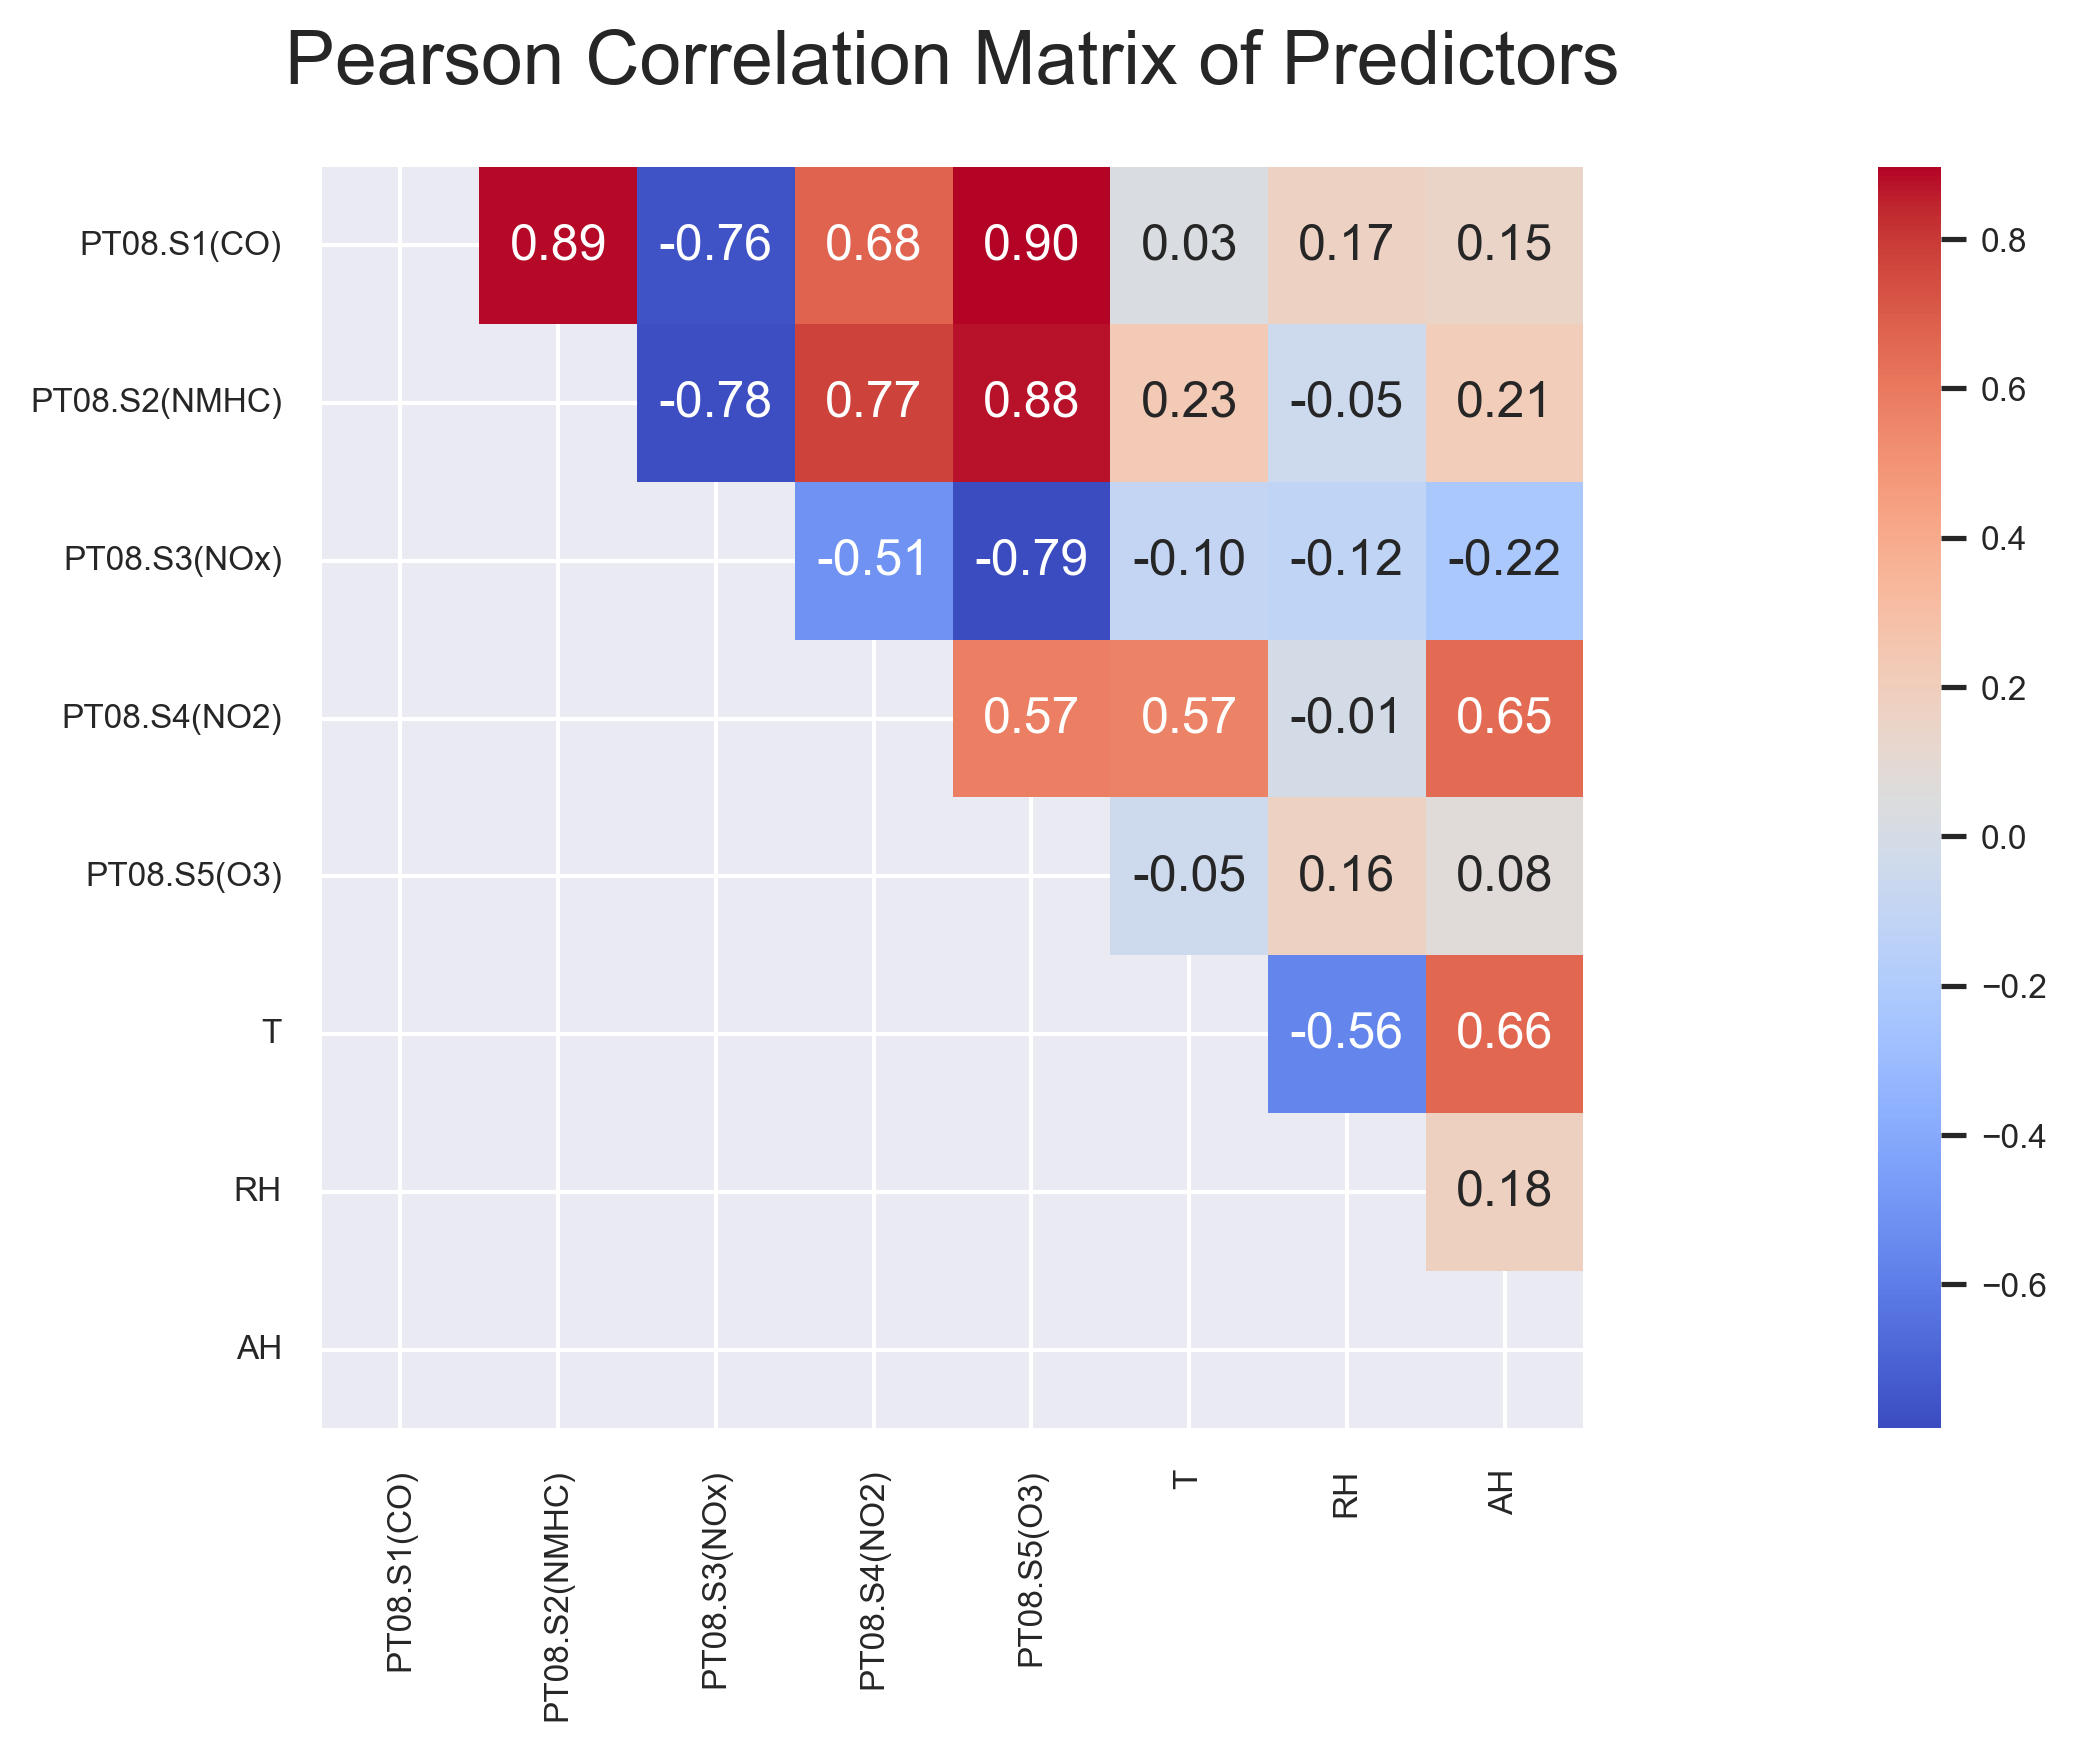
\includegraphics[width=0.75\linewidth]{figures/predictors_correlation_matrix.png}
    \caption{Matriz de correlação de Pearson entre preditores. Observa-se multicolinearidade forte entre leituras de sensores e correlações relevantes com umidade, motivando redução de dimensionalidade e/ou métodos penalizados.}
    \label{fig:corr}
\end{figure}

\paragraph{Pairplots e interações.}
As figuras de pares documentam relações bivariadas e separação por período do dia, evidenciando dependências não triviais e efeito temporal na dispersão.

\begin{figure}[htbp]
    \centering
    \includegraphics[width=0.95\linewidth]{figures/pairplot_day_period_selected.png}
    \caption{Pairplot dos preditores colorido por \texttt{day\_period}. Há clusterização fraca entre períodos e mudanças de densidade entre manhã, tarde e noite.}
    \label{fig:pairplot_dayperiod}
\end{figure}

\subsection{Construção do índice de poluição e classes (detalhes)}
\label{sec:cpi}
\begin{enumerate}
    \item Remover linhas com \texttt{NaN} em \texttt{CO}, \texttt{NOx}, \texttt{NO2}, \texttt{C6H6};
    \item Calcular o z-score: \( z_{i} = (x_{i}-\mu_{i})/\sigma_{i} \);
    \item Definir \( \mathrm{CPI} = \tfrac{1}{4}\sum_{i} z_{i} \);
    \item Discretizar o CPI em três quantis para obter \{\textit{Low}, \textit{Moderate}, \textit{High}\}.
\end{enumerate}

\subsection{Procedimentos estatísticos adicionais}
Calcularam-se estatísticas descritivas por classe e por recortes temporais (mês, dia da semana, período do dia). Para detecção exploratória de \emph{outliers} utilizou-se o limiar \( |z|>3 \); não houve remoção automática sem inspeção.
